\section{Introduction}

\subsection{Motivation}
The polyadenylation signal (PAS) is part of the 3' untranslated region(UTR) of almost every messenger RNA (mRNA). It is the binding site for a protein complex that causes the formation of the polyadenylation tail(poly(A)-tail). This tail of adenosines prevents the degradation of the mRNA in the cytoplasm effectively affecting the half-life of a mRNA and thereby raising the chance to be translated into a protein by the ribosome. As such, variants that have an impact on the efficiency of the PAS are potentially pathogenic due to their interference with the gene expression. Chen et al. wrote a review about diseases caused by PAS-affecting mutations. \todo{reference needed} 

Prediction of polyadenylation sites has been attempted several times with moderate success in the last twenty years. \todo{reference and example needed} Seeing that we cannot predict PASs with high accuracy prompts the question if we have enough knowledge about the structure of polyadenylation sites. Analyzing the secondary structure of the 3' UTR might give us more insight and allows the use of more characteristics for an accurate prediction.

Accurately identifying functional PASs enables us to detect disease-causing mutations easier or helps in gene prediction.  


\subsection{Aim}
The aim is to analyze the effect of mRNA base pair probabilities (BPP) on the prediction accuracy of functional, human polyadenylation signals. If possible, we want to improve the prediction accuracy since we assume that a consverved secondary structure is necessary for the polyadenylation process to work. The BPPs should reflect this conserved secondary structure at the polyadenylation signal sites.

 
\subsection{Existing tools}
There is a large pool of available methods and programs to predict functional polyadenylation sites. The majority of them rely on machine learning algorithms like neural network \citep{pmid8867844}, Hidden Markov Model \citep{pmid11937640, pmid15247332}, linear discriminant function \citep{pmid9088705}, quadratic discriminant function \citep{pmid10231571}, Support Vector Machine \citep{pmid15706523, pmid16870936} or Random Forest \citep{pmid23616439}. But other options are also available, e.g. position weight matrix \citep{pmid12600277} and fuzzy logic \citep{pmid19393560}.

The afore-mentioned methods and programs usually utilize the base composition surrounding the polyadenylation site to distinguish a functional PAS from a non-functional one. Almost all programs achieve moderate prediction accuarcies of 50\% to 60\%, leaving room for improvement. Since RNA secondary structure is becoming more and more the focus of scientific attention, incorporating features of secondary structure prediction might improve the accuracy to predict functional polyadenylation sites.   

\subsection{Background}

\subsubsection{Polyadenylation}
\label{Polyadenylation}
Polyadenylation (poly(A)) takes place in the cell nucleus and describes the process of adding adenosines to the 3' end of precursor mRNA (pre-mRNA), i.e. messenger RNA that has been recently transcribed and has yet to undergo any post-transcription steps like splicing or polyadenylation. Most eukaryotic mRNAs have a polyadenylated tail, except for histone mRNAs. \todo{reference needed, use the one from wiki "polyadenylation"}

After the transcription of the pre-mRNA by the RNA polymerase II the new transcript is cleaved and then polyadenylated. Cleavage is mediated by the enzyme complex cleavage and polyadenylation specificity factor (CPSF) which binds to the polyadenylation signal (PAS) sequence about 10 to 50 nucleotides upstream of the cleavage site. \todo{reference needed}The canonical PAS motif in humans is AAUAAA but there exist at least ten variants which bind less potently to CPSF. The motif sequence is also dependent on the taxonomic group, e.g. fungi and humans have a different canonical PAS motif. \todo{reference needed}

CPSF is usually assisted by two other protein complexes called cleavage stimulation factor (CstF) and cleavage factor I (CFI). CstF binds to a U/GU-rich region downstream of the cleavage site, the downstream sequence element (DSE), while CFI binds to a uracil-rich region upstream of the PAS, the upstream sequence element (USE). The presence of these two proteins greatly enhances the efficiency of the cleavage that occurs around 10 to 50 nucleotides downstream of the PAS.

After the cleavage CPSF recruits the poly(A) polymerase enzyme which is responsible for the addition of the adenosines at the cleavage site, resulting in the poly(A) tail. The length of the poly(A) tail is usually 200 to 250 adenosines long in mammals and differs in other taxonomic groups. Yeast, for example, only has a 80 nucleotides long poly(A) tail. The length of the tail is important for the survival of the mRNA, the shorter it is the more likely the mRNA is going to be degraded. Thus, the tail influences the half-life of a mRNA and with that the chance of the mRNA to be translated into a protein. \todo{reference needed}

\subsubsection{Alternative polyadenylation}
\label{apa}
The presence of multiple polyadenylation sites in one transcript is termed alternative polyadenylation (APA). It is a common occurence with at least half of human transcripts exhibiting this phenomenon. \citep{pmid23774734} Messenger RNAs from the same transcript can have identical coding sequence (CDS) but varying 3' UTR lengths, although uncommon, the coding sequence can be affected by APA causing another protein to be translated. \todo{reference needed}

\citeauthor{pmid23774734} differentiate between four classes of APA: tandem 3'UTR APA, alternative terminal exon APA, intronic APA and internal exon APA (see Fig. \ref{four_types_of_APA}) The most common class is tandem 3' UTR APA which is responsible for mRNAs with identical CDS but different 3' UTRs lengths, as described earlier. The other three APA classes will potentially create mRNAs with differing CDSs and are much rarer than tandem 3' UTR APA. 

We can conclude that tandem 3' UTR is a mechanism to regulate the expression of a protein by altering the length of its corresponding mRNAs' 3'UTRs, which is a docking platform for various inhibitiory factors like miRNAs. The other three classes, on the other hand, allow for more gene functionality since APA events are able to alter the CDS of mRNAs of one transcript and therefore, enable the translation of proteins with different functions.

\begin{figure}[ht]
	\centering
	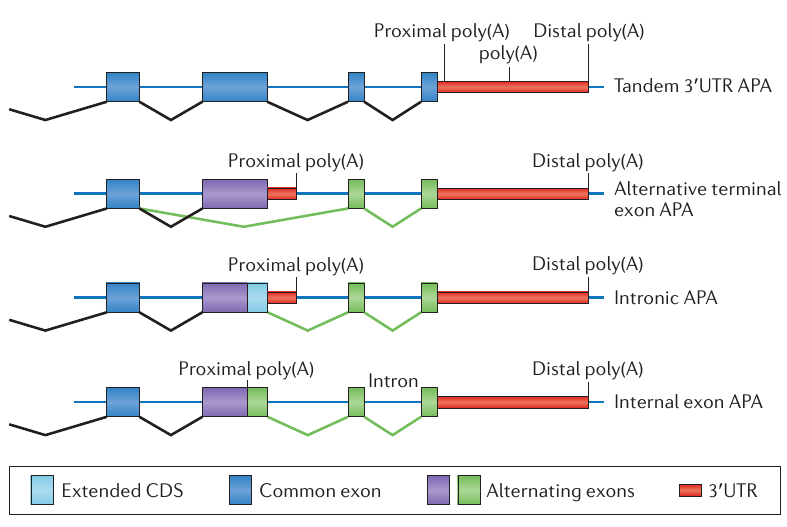
\includegraphics[width=1.0\textwidth]{pictures/four_types_of_APA.png}
	\caption{insert shitty text here}
	\label{four_types_of_APA}
\end{figure}

\subsubsection{Scientific history of polyadenylation}
\label{polyaHistory}
The enzyme polyadenylate polymerase which catalyzes the polyadenylation reaction was first discovered in 1960. \citep{pmid13819354} But the protein's function was revealed about a decade later. \citep{pmid5288383} At that time it was still a mystery why most mRNAs have polyadenylated tails. 

In the early 1980s the role of the poly(A)-tail was largely elucidated: nuclear export, translation and stability of the mature mRNA. (reviewed in \citep{pmid6111419}). 

It took another decade to discover the two primary proteins that mediate the 3' end cleavage and polyadenylation, namely CPSF and CStF. The number of participating proteins has since increased and recent publications mention several dozen cis-acting and auxiliary proteins or polypeptides working together in a large complex. \citep{pmid23774734} 

2008 it became clear that most genes have more than one polyadenylation site, resulting in transcripts with different lengths but identical coding sequence. \citep{pmid18411206} The new finding was termed alternative polyadenylation (APA). Since APA influences the length of the 3' untranslated Region (3' UTR), it is part of gene expression because the longer the 3' UTR the more binding sites for mRNA-repressive micro RNAs (miRNA) a transcript can have. \citep{pmid18566288}


\subsection{Messenger ribonucleic acid (mRNA)}
\label{mrna}
RNA is a molecule present in all lifeforms. There are many types of RNA like transfer RNA, ribosomal RNA, microRNA or messenger RNA. Most RNA types play key roles in coding (mRNA), decoding (tRNA), regulation (microRNA) and expression of genes.

mRNA is particularly interesting because it transports genetic information stored by the DNA to the protein synthesis factories of a cell, the ribosome. There, the mRNA specifies the amino acids sequence of a protein, making it an important component of the gene expression.

Every mRNA is composed of three parts: the 5' untranslated region (5' UTR), the coding sequence (CDS) and the 3' untranslated region (3' UTR). \todo{picture of mRNA structure} 

The 5' UTR is described as the region upstream of the start codon. It contains structures to regulate the translation of the transcript, like the 5' guanine cap. Although, it is called UTR, the 5' UTR may contain upstream open reading frames translating to peptides that inhibit the translation of the CDS of the transcript.

The CDS contains the sequence that is translated into an amino acid polymer by the ribosome.

The 3' UTR is defined as the region downstream of the stop codon. Because my thesis is focused on this region, it has a section of its own. (see \ref{3_UTR})

Messenger RNA is generated by the RNA polymerase II protein during the transcription process of a protein-coding gene. While prokaryotic and archaeal mRNA are rarely modified, eukaryotic mRNA is usually subject to many processing steps, including the addition of a 5' cap, splicing and polyadenylation. To distinguish between nascent and processed mRNA, the literature has termed them precursor mRNA and mature mRNA correspondingly.

The 5' cap is a special guanine that is added co-transcriptionally to the 5' end of a mRNA. It is needed for the transport of the mRNA from the nucleus to the cytoplasm and prevents the degradation by exonucleases. The cap is also important for the initiation of the translation in the ribosome. 

Splicing takes place during or after transcription and is responsible for the removal of the introns and the joining of the exons of most eukaryotic pre-mRNAs. Splicing can create different mRNAs and thus different proteins from the same pre-mRNA. 

Polyadenylation occurrs right after the cleavage of the transcript and describes the process of adding adenosines at the 3' end of the mRNA.\todo{reference needed}


\subsubsection{3' UTR}
\label{3_UTR}
The three prime untranslated region is usually part of the terminal exon of a transcript and starts where the coding sequence ends. It can span over several exons but that is uncommon. The length of the 3' UTR is quite variable in humans and can range from 60 to 4000 nucleotides. However, the average size is about 800 nucleotides. Another often analyzed feature is the mean GC-content which is 45\% for 3' UTRs of vertebrates. These characteristics differentiate the 3' UTR from the 5' UTR, which is on average only 200 nucleotides long and has a mean GC-content of about 60\%.\todo{3' utr, source [3]}

Although the 3'UTR is not translated into a protein, it contains many regulatory elements and regions which affect the translation efficency, localization and stability of the mRNA. 

One of these regulatory elements are miRNA response elements (MREs). Micro RNAs are about 20 nucleotides long and usually have an inhibitory effect on mRNA by inducing degradation of the mRNA, thus affecting translation efficeny. 

Like MREs, AU-rich elements (ARE) have a similar function. AREs are 50 to 150 nucleotides long and contain multiple copies of the sequence AUUUA. AREs can have inhibitory or enhancing effects but usually, like miRNA, they reduce the probability of translation by inducing mRNA degradation.

The poly(A) tail is also part of the 3' UTR and is target of so-called poly(A) binding proteins (PABPs). PABPs are important for the translation, export and stability of an mRNA. They can also form a complex with proteins that bind to the 5' cap of the mRNA. The result is a circular mRNA which allows for easier translation initiation \todo{reference needed}. While the presence of the poly(A) tail promotes translation, the abscence of the tail usually leads to degradation by the exosome. 

As we can see the 3' UTR is an important part of gene expression as it allows the cell to regulate the translation of proteins.


\subsection{RNA secondary structure prediction} 
Recently transcribed RNA molecules fold themselves into their mature conformation by forming complementary base pairings. Where complementary base pairings are not possible, loops emerge. Therefore, we can group RNA secondary structures into two categories: base pair stacks and loops (see Fig. \todo{pic to sec. structure types}). Knowing this, we can model secondary structure of an RNA molecule using graph theory: Each nucleotide of an RNA secondary structure is a node in a labeled graph. Adjacent nucleotides and nucleotides forming base pairs are connected by edges. These base pair edges are subject to the following restrictions:

\begin{enumerate}
	\item only Watson-Crick or GU base pairs are allowed;
	\item each node cannot have more than one base pair edge;
	\item the distance on the phosphate backbone between two base pairs must be at least three nucleotides;
	\item two base pair edges may not cross, i.e. if there is an edge $(i,j) \in G$ then there must not be an edge $(k,l) \in G$ with $i<k<j<l$ \todo{definition can allow edges to cross when k < i and i<l<j}.
\end{enumerate} 
The last restriction prohibits the formation of pseudoknots (see Fig. \todo{pic with sec. structures}), a secondary structure that is difficult to predict. It has been shown that the pseudoknot problem is NP-complete, rendering a solution computationally very costly. \citep{pmid22115189}

Most types of RNA have a distinctive three-dimensional structure like the hairpin structure of miRNAs or the cloverleaf structure of tRNA. In general, the secondary structure is more conserved than the underlying nucleic acid sequence which, for example, is relevant for phylogenetics (evolutionary history of species) or medical studies, since mutations can alter the structure of an RNA molecule, potentially causing diseases. \todo{reference needed} 

%RNA secondary structures are grouped into two categories: loops and stacks. A stack is a region of continuously paired bases and loops are further divided into internal loops, bulges, multiloops and external loops (see Fig \todo{figure of all loop types}).

In-silico prediction of RNA conformation is an ongoing and complex research subject as experimental elucidation of RNA structure is still expensive and time-consuming. Nowadays we can predict the secondary structure reasonably well but tertiary and quarternary structure still remain difficult to predict accurately.

%It is possible to predict the secondary structure from a single nucleic acid sequence or we can predict a consensus structure from multiple homologous nucleic acid sequences. The latter is also called comparative secondary structure prediction.
\subsubsection{Single sequence secondary structure prediction}
Experimental determination of molecule structure is often not feasible for the large amount of data DNA sequencers produce. For Bioinformaticians
this usually means, that we need to predict the molecule structure given only its sequence. Predicting the exact spatial structure is difficult with the current state of research and usually we can retrieve relevant information just by looking at the secondary structures. 

%am besten einfach nussinov -> zuker übergang erzählen und auf die probleme mit nussinov hinweisen
\citeauthor{pmid6163133} were one of the first to introduce a dynamic programming algorithm to solve the RNA folding problem. The Nussinov algorithm tries to maximize the number of base pairs, however this approach often led to inaccurate predictions.   

A year later, \citeauthor{pmid6163133} published an algorithm that incorporates ideas from chemical thermodynamics to predict the most stable structure: the conformation of a mature molecule is most stable when its in the state of thermal equilibrium, i.e. in the state of minimum free energy (MFE). For RNA secondary structures the MFE is mainly determined by the sum of their hydrogen bonds and base stacks. The free energy values of base pair interactions \todo{picture maybe?} and loops have been measured experimentially and are used in a nearest neighbor model by most implementations of the Zuker algorithm.  

Zuker's algorithm uses two matrices $W(i,j)$ and $V(i,j)$. $W(i,j)$ denotes the minimum free energy of all structures that are formed by the subsequence $i$ to $j$, while $V(i,j)$ denotes the minimum free energy of all structures that are formed by the subsequence $i$ to $j$, if $i$ and $j$ are paired. The recursions for $W(i,j)$ are defined as follows:

\begin{equation*}
W(i,j) = min
\begin{cases}
	W(i+1,j) \\
	W(i,j-1) \\
	V(i,j) \\
	min\{W(i,j)+W(k+1,j)\} \text{ where $i<k<j$}
\end{cases}
\end{equation*}

The equation differentiates between four cases (top to bottom): $i$ is unpaired, $j$ is unpaired, $i$ and $j$ form a base pair and $i$ and $j$ form base pairs but not with each other. When $i$ and $j$ form a base pair we differentiate again between four cases by using the following equation:

\begin{equation*}
V(i,j) = min
\begin{cases}
	eH(i,j) \\
	eS(i,j) + v(i+1,j-1) \\
	min[eL(i,j,i',j') + V(i',j')] & \text{ where $i<i'<j'<k$} \\
	min[W(i+1,k)+W(k+1,j-1)] & \text{ where $i+1<k<j-1$}
\end{cases}
\end{equation*}

Here, $eH$ calculates the energy of a hairpin loop spanning from $i$ to $j$, $eS$ is the energy of $i$ and $j$ being part of a base stack, the third case calculates the energy of a bulge or interior loop and the last case calculates the energy used for the formation of a multiloop.

The MFE of the whole sequence is then determined by $W(1,n)$ for a $n$ nucleotides long sequence. The time complexity is $O(n^4)$ but can be improved to $O(n^3)$ by setting a limit to the maximum size of an interior loop (usually set to 30).   

RNA secondary structure is usually more accurately predicted by the Zuker algorithm compared to the Nussinov algorithm. And although Zuker's approach is widely used nowadays there are a few issues:
\begin{itemize}
	\item Pseudoknots cannot be detected by Zuker;
	\item The nearest neighbor model used to calculate the free energies is not precise enough;
	\item Some known RNAs do not fold themselves into their possible MFE structure;
	\item Some RNAs have more than one biologically active conformation.
\end{itemize}

While the pseudoknot problem is not efficiently solvable, the other three issues can be alleviated by taking a look at suboptimal structures, i.e. conformations that are equal or close to the MFE conformation. Many software packages allow the prediction of suboptimal structures. 

 
\subsubsection{Comparative secondary structure prediction}
The basic idea behind comparative structure analysis is that important structural elements are usually highly conserved. Consequential\todo{consequentially?}, homologous sequences are likely to fold similarily. We want to extract information from the secondary structure conserveration using multiple sequence alignemnts (MSAs). This means that we are not exactly predicting the secondary structures of a single molecule but a consensus secondary structure. There are three common methods available: 


\subsubsection{McCaskill algorithm - calculating BPPs}
In 1990 \citeauthor{pmid1695107} introduced an algorithm to compute the partition function of a single stranded nucleic acid sequence. The partition function is a method orginating from  mechanical statistics to calculate the likelihood of observing a certain state in a thermodynamic system. The states a system can adopt is called the ensemble. The partition function $Q$ for the ensemble of all possible secondary structures $S$ is defined as follows\citep{pmid1695107}:  

\begin{equation*}
	Q = \sum_{S} e^{-\dfrac{\Delta G(S)}{RT}}
\end{equation*} \\
where
\begin{equation*}
  \begin{aligned}
	T &= \text{temperature in Kelvin} \\
	\Delta G &= \text{change in the Gibbs free energy} \\
	R &= \text{ideal gas constant}
  \end{aligned}
\end{equation*}

With the help of the partition function we can calculate the probability of a base pair $(k,l)$ forming in the ensemble. Analogous to the Zuker algorithm, McCaskill differentiates between several cases:

\begin{enumerate}
	\item $(k,l)$ is a non-enclosed base pair, i.e. there is no base pair $(i,j)$ where $k<i<j<l$;
	\item $(k,l)$ is a bulge, interior loop or part of a stack with $(i,j)$;
	\item $(k,l)$ is an inner base pair of a multiloop closed by $(i,j)$
\end{enumerate}



\subsubsection{ViennaRNA}
The Vienna RNA Package\todo{reference needed} is a widely used library for RNA folding written in the programming language C. The first version was released in 1994 and offered the calculation of the MFE structure or the partition function. The package is shipped with several standalone CLI programs like RNAfold or RNAalifold. 


